
\documentclass[11pt,a4paper]{report}

\usepackage[portuges]{babel}
\usepackage[utf8]{inputenc} % define o encoding usado texto fonte (input)--usual "utf8" ou "latin1
\usepackage{graphicx} %permite incluir graficos, tabelas, figuras
\usepackage{subcaption}
\usepackage{listings}
\usepackage{color}
\usepackage{multicol}
\usepackage{indentfirst}
\usepackage{hyperref}
\usepackage{amsmath}
\usepackage{amssymb}
\usepackage{float}
\usepackage{enumitem}

\newlist{SubItemList}{itemize}{1}
\setlist[SubItemList]{label={$-$}}

\let\OldItem\item
\newcommand{\SubItemStart}[1]{%
    \let\item\SubItemEnd
    \begin{SubItemList}[resume]%
        \OldItem #1%
}
\newcommand{\SubItemMiddle}[1]{%
    \OldItem #1%
}
\newcommand{\SubItemEnd}[1]{%
    \end{SubItemList}%
    \let\item\OldItem
    \item #1%
}
\newcommand*{\SubItem}[1]{%
    \let\SubItem\SubItemMiddle%
    \SubItemStart{#1}%
}%

\definecolor{myblue}{rgb}{0.2,0.2,0.8}
\definecolor{mygray}{rgb}{0.5,0.5,0.5}
\definecolor{mymauve}{rgb}{0.58,0,0.82}

\lstdefinestyle{code}{ 
  backgroundcolor=\color{white},   % choose the background color; you must add \usepackage{color} or \usepackage{xcolor}; should come as last argument
  basicstyle=\footnotesize,        % the size of the fonts that are used for the code
  breakatwhitespace=false,         % sets if automatic breaks should only happen at whitespace
  breaklines=true,                 % sets automatic line breaking
  captionpos=b,                    % sets the caption-position to bottom
  commentstyle=\color{white},    % comment style
  deletekeywords={...},            % if you want to delete keywords from the given language
  escapeinside={\%*}{*)},          % if you want to add LaTeX within your code
  extendedchars=true,              % lets you use non-ASCII characters; for 8-bits encodings only, does not work with UTF-8
  firstnumber=1000,                % start line enumeration with line 1
  keepspaces=true,                 % keeps spaces in text, useful for keeping indentation of code (possibly needs columns=flexible)
  keywordstyle=\color{blue},       % keyword style
  language=C++,                 % the language of the code
  morekeywords={*,...},            % if you want to add more keywords to the set
  numberstyle=\tiny\color{mygray}, % the style that is used for the line-numbers
  rulecolor=\color{black},         % if not set, the frame-color may be changed on line-breaks within not-black text (e.g. comments (green here))
  showspaces=false,                % show spaces everywhere adding particular underscores; it overrides 'showstringspaces'
  showstringspaces=false,          % underline spaces within strings only
  showtabs=false,                  % show tabs within strings adding particular underscores
  stepnumber=2,                    % the step between two line-numbers. If it's 1, each line will be numbered
  stringstyle=\color{mymauve},     % string literal style
  tabsize=2,	                   % sets default tabsize to 2 spaces
  title=\lstname                   % show the filename of files included with \lstinputlisting; also try caption instead of title
}

\title{Sistemas Operativos - Trabalho Prático\\
       \textbf{Grupo 17}\\ Relatório
       } %Titulo do documento
%\title{Um Exemplo de Artigo em \LaTeX}
\author{Inês Pires Presa\\ (A90355)\and Ivo Miguel Gomes Lima\\ (A90214)\and Tiago dos Santos Silva Peixoto Carriço \\ (A91695)
       } %autores do documento
\date{\today} %data

\begin{document}
	\begin{minipage}{0.9\linewidth}
        \centering
		
\includegraphics[width=0.4\textwidth]{um.jpeg}\par\vspace{1cm}
                \href{https://www.uminho.pt/PT}
		{\scshape\LARGE Universidade do Minho} \par
		\vspace{0.6cm}
                \href{https://lcc.di.uminho.pt}
		{\scshape\Large Licenciatura em Ciências da Computação} \par
		\maketitle
		\begin{figure}[H]
			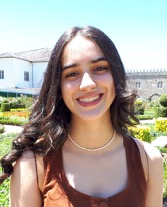
\includegraphics[width=0.32\linewidth]{ines.jpg}
			
\includegraphics[width=0.32\linewidth]{ivo.jpg}
			
\includegraphics[width=0.32\linewidth]{tiago.jpg}
		\end{figure}
	\end{minipage}

\tableofcontents % insere Indice

\chapter{Introdução}

Foi-nos proposto, no âmbito da unidade curricular de Sistemas Operativos, o desenvolvimento de um sistema capaz de transformar vários ficheiros de áudio concorrentemente, consultar as tarefas em execução, mostrando ainda o número de filtros disponiveis e em uso nessas transformações. Este tipo de sistema utiliza um conjunto de executáveis para filtrar e modificar um fluxo de áudios, permitindo tratar grandes quantidades de dados explorando a concorrência entre os diferentes processos.

Neste relatório, vamos explicitar a nossa abordagem ao problema, justificando a estrutura do nosso sistema e demonstrar os conhecimentos adquiridos durante as aulas, tais como a utilização/criação de processos, duplicação de descritores, criação de \emph{pipes} sem/com nome, execução de processos, aplicação de sinais e \emph{system calls}.

Primeiramente, descreveremos as funcionalidades que o nosso programa suporta e, de seguida, faremos uma breve caracterização do nosso código, referindo a arquitectura de processos e os mecanismos de comunicação utilizados.

\chapter{Funcionalidades}

\section{Aplicação de Filtros}

Submetendo um comando do tipo \emph{./aurras transform}, seguido dos nomes do ficheiro original assim como do ficheiro processado e de uma sequência de identificadores de filtros, o programa aplica-os ao primeiro ficheiro, guardando o resultado final no segundo. Esta ação só não será efetuada caso seja pedido que algum dos filtros seja aplicado um número de vezes superior ao máximo definido no ficheiro de configuração. Quando esse valor é alcançado devido à pré-existência de pedidos, este fica em lista de espera para que possa ser posteriormente processado.

\section{Verifição do Estado}

Caso o comando seja do tipo \emph{./aurras status}, o cliente recebe do servidor uma descrição dos pedidos que estão a ser processados, assim como uma lista dos filtros em utilização e a identificação do \emph{pid} do servidor.

\section{Informação de Utilização}

Na eventualidade de o utilizador pretender obter informação relativa às funcionalidades suportadas pelo cliente (servidor), este terá de digitar \emph{./aurras} (\emph{./aurrasd}). 

\chapter{Estrutura de implementação}

\section{Cliente (\emph{aurras.c})}

Para a implementação das funcionalidades referidas anteriormente, foi necessário a criação de duas funções \emph{status} e \emph{transform} que serão brevemente descritas de seguida.

\begin{itemize}
\item \textbf{Status: } São criados dois \emph{pipes} com nome que fazem a ligação com o servidor. O \emph{pipe\_escrever} é empregue para o envio do pedido de verificação do estado conduzido pelo cliente, em contrapartida o \emph{pipe\_ler} recebe a informação solicitada, que será imprimida no \emph{standard output}. O \emph{pid} do cliente é enviado através do \emph{pipePrincipal} para o servidor.
\item \textbf{Transform: } Nesta função só é criado um \emph{pipe\_escrever}, uma vez que o método de comunicação que definimos no sentido servidor -\textgreater cliente é a utilização de sinais. Desta forma, o \emph{pipe} é utilizado para enviar a informação referente ao pedido de transformação do ficheiro e quando o processo é iniciado o cliente recebe um sinal (\emph{SIGUSR1}).
\end{itemize}

\section{Servidor (\emph{aurrasd.c})}

\subsection{Variáveis Globais}

\begin{itemize}
\item \textbf{Filtro filtros: } Esta variável dá acesso à \emph{struct lligada} que serve para armazenar as informações presentes no ficheiro de configuração, nomeadamente  o nome do filtro, o nome do executável e o número máximo de uso simultâneo desse filtro, para além disso guarda também o número de utilizações, no momento, do mesmo.
\item \textbf{Task tasks: } Esta variável tem uma estrutura de dados que lhe é associada, sendo esta responsável por guardar uma lista de \emph{tasks}, armazenando em cada \emph{nodo} o conjunto de dados necessários para processar uma determinada \emph{task} (comando usado para a invocar, nome dos filtros pela ordem que devem ser aplicados, nome de cada filtro e respetiva quantidade de vezes que deve ser executado, número da task, estado do processameno, \emph{pid} do processo filho responsável pelo processamento do pedido, nome do ficheiro original e nome do ficheiro processado).
\item \textbf{char* pasta\_filtros: } Nome da diretória onde se encontram os ficheiros de filtros. 
\item \textbf{int numero\_tasks:} Número de tasks recebidas até ao momento.
\end{itemize}

\subsection{Descrição do Funcionamento}

O servidor começa por testar se na sua inicialização recebeu os três argumetos necessários para o seu funcionamento. Caso isso se verifique, passa então à criação de um pipe que estabelecerá a comunicação entre o servidor e os clientes.

De seguida, é informado, através desse \emph{pipe} do \emph{pid} do cliente, para que possa tomar conhecimento do \emph{pipe\_lercliente} que traz a indicação da tarefa que deve ser efetuada. Caso esta tarefa seja um pedido de verificação do estado, será chamada a função \emph{status}, caso seja uma requisição de transformação de ficheiro de áudio, será invocada a função \emph{transform}. Este processo será repetido até que seja recebido um sinal de \emph{SIGINT} ou \emph{SIGTERM} que fechará de forma elegante o servidor. A seguir serão descritas as funções referidas.

\begin{itemize}
     \item{\textbf{Status: } Começa por criar um processo filho, que enviará através do \emph{pipe\_escrever} a informação do estado atual do programa ao cliente.}
     \item{\textbf{Transform: } No momento inicial armazena a informação referente ao pedido na estrutura de dados criada para o efeito (\emph{tasks}), de seguida, verifica se o pedido pode ser executado utilizando a função \emph{disponibilidade}. Em função do \emph{output} da função referida, será tomado um de três caminhos:}
     \begin{itemize}
     \item{O pedido é descartado (-1).}
     \item{ O pedido é colocado em espera (0).}
     \item{O pedido é executado (1).}
     \end{itemize}
     Passamos agora a explicar a arquitetura de processos adotada para a execução da transformação de um ficheiro: é criado um processo filho para monitorizar as operações, sendo que de seguida cria-se um outro processo filho dentro do \emph{monitor} que será responsável pela criação dos processos que executarão a aplicação dos filtros.
\end{itemize}

\newpage

\begin{figure}[h]
    \centering
    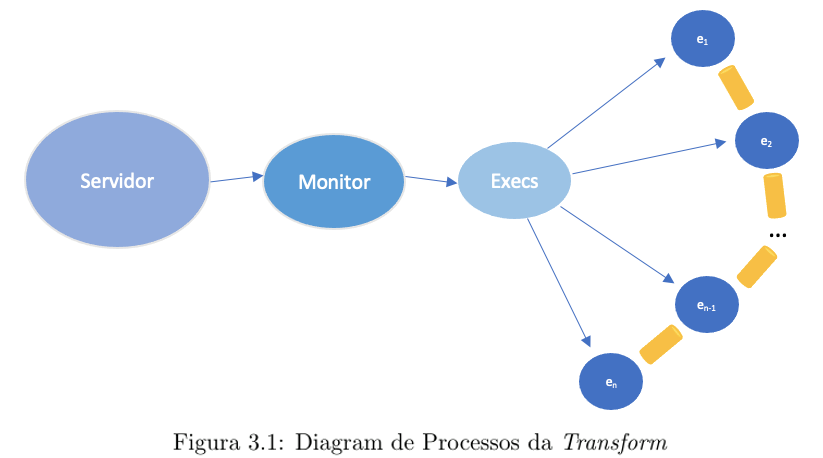
\includegraphics[width=1\textwidth]{diagrama}
\end{figure}

\chapter{Conclusão}

Durante a realização deste trabalho prático, embora o mesmo tenha sido apelidado de simples e até mesmo básico por parte da equipa docente, sentimos a necessidade de uma grande organização da nossa parte para que não fosse perdido o foco do problema que estavamos a enfrentar. A aplicação dos conceitos teóricos revelou-se, de uma maneira geral, bastante interessante e desafiante pois tal como \emph{\textbf{Ward Cunningham}} disse \emph{\textbf{It's all talk until the code runs}}. 

Uma das peças fundamentais para a concretização do projeto foram as resoluções dos guiões práticos apresentadas pela equipa docente e até mesmo as nossas, pois serviram de apoio para o esclarecimento de dúvidas que surgiram, o que nos permitiu finalizar o mesmo com todas as funcionalidades solicitadas. Consideramos que a maior dificuldade foi sentida no momento inicial, sendo o principal obstáculo a visualização do produto final para a nossa abordagem ao problema, mas conforme foram estabelecidos \emph{mini checkpoints} conseguimos ultrapassar este impasse e suceder com uma boa implementação.

\end{document}